\documentclass[11pt,a4paper]{article}

% --- Core Packages ---
\usepackage[utf8]{inputenc}
\usepackage[T1]{fontenc}
\usepackage{amsmath, amssymb, amsfonts, amsthm}
\usepackage{physics}
\usepackage{graphicx}
\usepackage{tcolorbox}
\usepackage{longtable}
\usepackage{booktabs}
\usepackage{geometry}
\usepackage{enumitem}
\usepackage{fancyhdr}

% --- TikZ Setup for Diagrams ---
\usepackage{tikz}
\usetikzlibrary{arrows.meta, positioning, calc}

% --- Geometry Settings ---
\geometry{
    top=1.0in,
    bottom=1.0in,
    left=0.85in,
    right=0.85in,
    headheight=14pt
}

% --- Custom Colors ---
\definecolor{RoyalBlue}{rgb}{0.08, 0.35, 0.65}
\definecolor{dimgray}{rgb}{0.41, 0.41, 0.41}
\definecolor{ForestGreen}{rgb}{0.10, 0.55, 0.20}

\pagestyle{fancy}
\fancyhf{}
\fancyhead[L]{\color{dimgray}\itshape Electricity \& Magnetism --- Important Derivations Register}
\fancyhead[R]{\color{dimgray}\itshape Revision Guide}
\fancyfoot[C]{\thepage}
\renewcommand{\headrulewidth}{0.4pt}

\begin{document}

\title{\textbf{\Huge Electricity \& Magnetism}\\[0.4cm]
\Large Option B: Important Derivations Register}
\author{\textbf{Exam Revision Version}}
\date{\today}
\maketitle

\tableofcontents
\newpage

% =========================================================================
% DERIVATION 1
% =========================================================================
\section{Derivation 1: Gauss's Theorem (Most Important)}

\subsection*{PYQ Weightage}
\begin{tcolorbox}[colback=yellow!10!white, colframe=orange, halign=center]
    \textbf{PYQ Weightage: \textasteriskcentered\textasteriskcentered\textasteriskcentered\textasteriskcentered\textasteriskcentered}
\end{tcolorbox}

\subsection*{Question}
State and prove Gauss's theorem in electrostatics.

\subsection*{Statement}
The total electric flux through any closed surface is equal to \( \frac{1}{\epsilon_0} \) times the total charge enclosed within the surface.

\subsection*{Diagram}
\begin{center}
    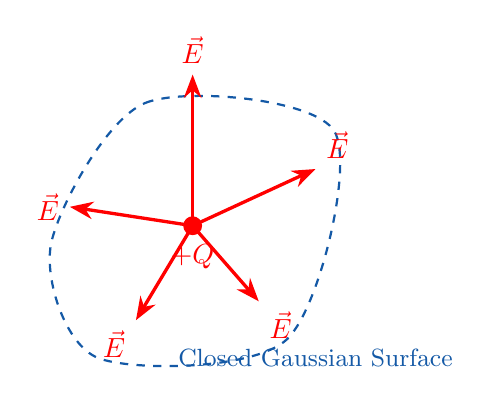
\begin{tikzpicture}[>=Stealth, thick, scale=1.2]
        % Outer Gaussian surface
        \draw [dashed, RoyalBlue] plot [smooth cycle] coordinates {(0,0) (1,1.5) (3,1.2) (2.5,-1) (0.5,-1.2)};
        % Charge Q in the middle
        \filldraw [red] (1.5,0.2) circle (2.5pt) node[below=3pt] {$+Q$};
        % Electric field vectors
        \draw [->, red, very thick] (1.5,0.2) -- (1.5,1.8) node[above] {$\vec{E}$};
        \draw [->, red, very thick] (1.5,0.2) -- (2.8,0.8) node[above right] {$\vec{E}$};
        \draw [->, red, very thick] (1.5,0.2) -- (0.2,0.4) node[left] {$\vec{E}$};
        \draw [->, red, very thick] (1.5,0.2) -- (0.9,-0.8) node[below left] {$\vec{E}$};
        \draw [->, red, very thick] (1.5,0.2) -- (2.2,-0.6) node[below right] {$\vec{E}$};
        \node [RoyalBlue] at (2.8,-1.2) {\small Closed Gaussian Surface};
    \end{tikzpicture}
\end{center}

\subsection*{Proof}
Consider a point charge \( Q \) enclosed inside a closed surface.
Electric field at a point on the surface:
\[ E = \frac{1}{4\pi\epsilon_0} \frac{Q}{r^2} \]

Small area element:
\[ dA \]

Electric flux through area element:
\[ d\phi = \vec{E} \cdot d\vec{A} \]
\[ d\phi = E \, dA \cos\theta \]

But
\[ d\Omega = \frac{dA \cos\theta}{r^2} \]
where \( d\Omega \) is the solid angle.

Hence
\[ d\phi = \frac{Q}{4\pi\epsilon_0} d\Omega \]

Integrating over complete closed surface,
\[ \phi = \frac{Q}{4\pi\epsilon_0} \int d\Omega \]

Total solid angle around a point:
\[ \int d\Omega = 4\pi \]

Therefore
\[ \phi = \frac{Q}{4\pi\epsilon_0} (4\pi) \]

\begin{tcolorbox}[colback=RoyalBlue!5!white, colframe=RoyalBlue]
    \[ \phi = \frac{Q}{\epsilon_0} \]
\end{tcolorbox}

\subsection*{Final Result}
\begin{tcolorbox}[colback=RoyalBlue!5!white, colframe=RoyalBlue]
    \[ \oint \vec{E} \cdot d\vec{A} = \frac{Q}{\epsilon_0} \]
\end{tcolorbox}

\subsection*{Differential Form}
Using Divergence Theorem,
\begin{tcolorbox}[colback=RoyalBlue!5!white, colframe=RoyalBlue]
    \[ \nabla \cdot \vec{E} = \frac{\rho}{\epsilon_0} \]
\end{tcolorbox}

\subsection*{Exam Ending Line}
Hence proved that the total electric flux through any closed surface equals the enclosed charge divided by \( \epsilon_0 \).

\newpage

% =========================================================================
% DERIVATION 2
% =========================================================================
\section{Derivation 2: Electric Field Due to Infinite Line Charge Using Gauss Law}

\subsection*{PYQ Weightage}
\begin{tcolorbox}[colback=yellow!10!white, colframe=orange, halign=center]
    \textbf{PYQ Weightage: \textasteriskcentered\textasteriskcentered\textasteriskcentered\textasteriskcentered\textasteriskcentered}
\end{tcolorbox}

\subsection*{Question}
Using Gauss's theorem, obtain the electric field due to an infinitely long straight line charge.

\subsection*{Diagram}
\begin{center}
    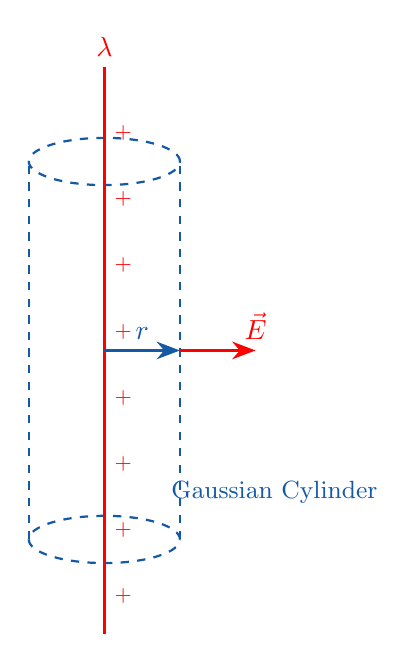
\begin{tikzpicture}[>=Stealth, thick, scale=1.2]
        % Draw cylinder
        \draw[dashed, RoyalBlue] (0,2) ellipse (0.8 and 0.25);
        \draw[dashed, RoyalBlue] (-0.8,-2) -- (-0.8,2);
        \draw[dashed, RoyalBlue] (0.8,-2) -- (0.8,2);
        \draw[dashed, RoyalBlue] (-0.8,-2) arc (180:360:0.8 and 0.25);
        \draw[dashed, RoyalBlue] (0.8,-2) arc (0:180:0.8 and 0.25);
        
        % Draw line charge
        \draw[very thick, red] (0,-3) -- (0,3) node[above] {$\lambda$};
        \foreach \y in {-2.6, -1.9, -1.2, -0.5, 0.2, 0.9, 1.6, 2.3} {
            \node[red, scale=0.8] at (0.2, \y) {$+$};
        }
        
        % Radius arrow
        \draw[->, RoyalBlue, very thick] (0,0) -- (0.8,0) node[midway, above] {$r$};
        \draw[->, red, very thick] (0.8,0) -- (1.6,0) node[above] {$\vec{E}$};
        \node [RoyalBlue] at (1.8,-1.5) {\small Gaussian Cylinder};
    \end{tikzpicture}
\end{center}

\subsection*{Given}
\begin{itemize}
    \item Linear charge density: \( \lambda \)
    \item Radius of Gaussian cylinder: \( r \)
    \item Length: \( l \)
\end{itemize}

\subsection*{Step 1}
Choose cylindrical Gaussian surface. By symmetry, the electric field is radial and constant over the curved surface.

\subsection*{Step 2: Apply Gauss Law}
\[ \oint E \, dA = \frac{Q}{\epsilon_0} \]

\subsection*{Step 3}
Flux through end caps = 0 because \( \vec{E} \perp d\vec{A} \).
Only curved surface contributes.
Curved surface area:
\[ A = 2\pi rl \]
Thus
\[ E(2\pi rl) = \frac{\lambda l}{\epsilon_0} \]

\subsection*{Step 4}
Cancel \( l \):
\[ E(2\pi r) = \frac{\lambda}{\epsilon_0} \]
Hence
\begin{tcolorbox}[colback=RoyalBlue!5!white, colframe=RoyalBlue]
    \[ E = \frac{\lambda}{2\pi\epsilon_0 r} \]
\end{tcolorbox}

\subsection*{Final Result}
\begin{tcolorbox}[colback=RoyalBlue!5!white, colframe=RoyalBlue]
    \[ E = \frac{\lambda}{2\pi\epsilon_0 r} \]
\end{tcolorbox}

\subsection*{Important Note}
\[ E \propto \frac{1}{r} \]

\subsection*{Exam Ending Line}
Hence the electric field due to an infinite line charge decreases inversely with distance.

% ---

% =========================================================================
% DERIVATION 3
% =========================================================================
\section{Derivation 3: Electric Potential Due to an Electric Dipole}

\subsection*{PYQ Weightage}
\begin{tcolorbox}[colback=yellow!10!white, colframe=orange, halign=center]
    \textbf{PYQ Weightage: \textasteriskcentered\textasteriskcentered\textasteriskcentered\textasteriskcentered\textasteriskcentered\ Direct PYQ (Set 1 \& Set 3)}
\ \end{tcolorbox}

\subsection*{Question}
Obtain an expression for the electric potential due to an electric dipole at a point \( P(r,\theta) \).

\subsection*{Diagram}
\begin{center}
    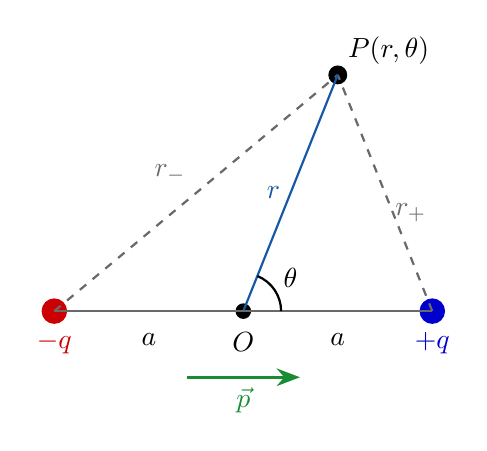
\begin{tikzpicture}[>=Stealth, thick, scale=1.2]
        % Charges
        \filldraw [red!80!black] (-2,0) circle (3.5pt) node[below=4pt] {$-q$};
        \filldraw [blue!80!black] (2,0) circle (3.5pt) node[below=4pt] {$+q$};
        \filldraw [black] (0,0) circle (2pt) node[below=4pt] {$O$};
        
        % Point P
        \filldraw [black] (1,2.5) circle (2.5pt) node[above right] {$P(r,\theta)$};
        
        % Lines from charges and center to P
        \draw [dashed, dimgray] (-2,0) -- (1,2.5) node[midway, above left] {$r_-$};
        \draw [dashed, dimgray] (2,0) -- (1,2.5) node[midway, below right] {$r_+$};
        \draw [thick, RoyalBlue] (0,0) -- (1,2.5) node[midway, left] {$r$};
        \draw [thick, dimgray] (-2,0) -- (2,0);
        
        % Angle theta
        \draw (0.4,0) arc (0:68:0.4);
        \node at (0.5,0.35) {$\theta$};
        
        % Labels
        \node at (-1,-0.3) {$a$};
        \node at (1,-0.3) {$a$};
        \draw [->, ForestGreen, very thick] (-0.6,-0.7) -- (0.6,-0.7) node[midway, below] {$\vec{p}$};
    \end{tikzpicture}
\end{center}

\subsection*{Given}
\begin{itemize}
    \item Dipole charges: \( -q, \quad +q \)
    \item Separation: \( 2a \)
    \item Dipole moment:
    \begin{tcolorbox}[colback=RoyalBlue!5!white, colframe=RoyalBlue]
        \[ p = 2aq \]
    \end{tcolorbox}
\end{itemize}

\subsection*{Step 1: Potential Due to Individual Charges}
Potential due to positive charge:
\[ V_+ = \frac{1}{4\pi\epsilon_0} \frac{q}{r_+} \]
Potential due to negative charge:
\[ V_- = -\frac{1}{4\pi\epsilon_0} \frac{q}{r_-} \]

\subsection*{Step 2: Total Potential}
By superposition,
\[ V = V_+ + V_- \]
\[ V = \frac{1}{4\pi\epsilon_0} \left( \frac{q}{r_+} - \frac{q}{r_-} \right) \]

\subsection*{Step 3: For a Distant Point}
When \( r \gg a \), we use
\[ r_+ = r - a\cos\theta \]
\[ r_- = r + a\cos\theta \]
Substituting,
\[ V = \frac{q}{4\pi\epsilon_0} \left[ \frac{1}{r - a\cos\theta} - \frac{1}{r + a\cos\theta} \right] \]

\subsection*{Step 4: Simplification}
Using
\[ \frac{1}{x-y} - \frac{1}{x+y} = \frac{2y}{x^2-y^2} \]
we obtain
\[ V = \frac{q}{4\pi\epsilon_0} \frac{2a\cos\theta}{r^2} \]
Since \( p = 2aq \), therefore
\begin{tcolorbox}[colback=RoyalBlue!5!white, colframe=RoyalBlue]
    \[ V = \frac{1}{4\pi\epsilon_0} \frac{p\cos\theta}{r^2} \]
\end{tcolorbox}

\subsection*{Final Result}
\begin{tcolorbox}[colback=RoyalBlue!5!white, colframe=RoyalBlue]
    \[ V = \frac{1}{4\pi\epsilon_0} \frac{p\cos\theta}{r^2} \]
\end{tcolorbox}

\subsection*{Special Cases}
\subsubsection*{Axial Position (\( \theta = 0^\circ \))}
\begin{tcolorbox}[colback=RoyalBlue!5!white, colframe=RoyalBlue]
    \[ V = \frac{1}{4\pi\epsilon_0} \frac{p}{r^2} \]
\end{tcolorbox}

\subsubsection*{Equatorial Position (\( \theta = 90^\circ \))}
\begin{tcolorbox}[colback=RoyalBlue!5!white, colframe=RoyalBlue]
    \[ V = 0 \]
\end{tcolorbox}

\subsection*{Exam Ending Line}
Hence the electric potential due to a short dipole at a distant point is
\begin{tcolorbox}[colback=RoyalBlue!5!white, colframe=RoyalBlue]
    \[ V = \frac{1}{4\pi\epsilon_0} \frac{p\cos\theta}{r^2} \]
\end{tcolorbox}

\newpage

% =========================================================================
% DERIVATION 4
% =========================================================================
\section{Derivation 4: Electric Field Due to an Electric Dipole}

\subsection*{PYQ Weightage}
\begin{tcolorbox}[colback=yellow!10!white, colframe=orange, halign=center]
    \textbf{PYQ Weightage: \textasteriskcentered\textasteriskcentered\textasteriskcentered\textasteriskcentered\textasteriskcentered\ Direct PYQ (Set 1 \& Set 3)}
\end{tcolorbox}

\subsection*{Question}
Obtain expressions for electric field due to an electric dipole on:
\begin{enumerate}
    \item Axial position
    \item Equatorial position
\end{enumerate}

\subsection*{(A) Electric Field on Axial Line}
\subsubsection*{Diagram}
\begin{center}
    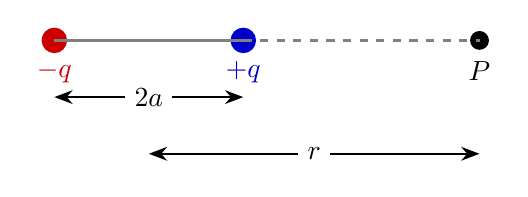
\begin{tikzpicture}[>=Stealth, thick, scale=1.2]
        % Charges
        \filldraw [red!80!black] (-2,0) circle (3.5pt) node[below=4pt] {$-q$};
        \filldraw [blue!80!black] (0,0) circle (3.5pt) node[below=4pt] {$+q$};
        % Line
        \draw [thick, gray] (-2,0) -- (0,0);
        \draw [<->] (-2,-0.6) -- (0,-0.6) node[midway, fill=white] {$2a$};
        
        % Point P
        \filldraw [black] (2.5,0) circle (2.5pt) node[below=4pt] {$P$};
        \draw [dashed, gray] (0,0) -- (2.5,0);
        
        % Distance r
        \draw [<->] (-1,-1.2) -- (2.5,-1.2) node[midway, fill=white] {$r$};
    \end{tikzpicture}
\end{center}

\subsubsection*{Step 1}
Field at \( P \) due to \( +q \):
\[ E_+ = \frac{1}{4\pi\epsilon_0} \frac{q}{(r-a)^2} \]
Direction: Right

\subsubsection*{Step 2}
Field due to \( -q \):
\[ E_- = \frac{1}{4\pi\epsilon_0} \frac{q}{(r+a)^2} \]
Direction: Left

\subsubsection*{Step 3}
Net Field:
\[ E = E_+ - E_- \]
\[ E = \frac{q}{4\pi\epsilon_0} \left[ \frac{1}{(r-a)^2} - \frac{1}{(r+a)^2} \right] \]

\subsubsection*{Step 4}
Simplifying,
\[ E = \frac{1}{4\pi\epsilon_0} \frac{4aqr}{(r^2-a^2)^2} \]
For \( r \gg a \),
\[ r^2 - a^2 \approx r^2 \]
Therefore
\[ E = \frac{1}{4\pi\epsilon_0} \frac{4aq}{r^3} \]
Since \( p = 2aq \),
\begin{tcolorbox}[colback=RoyalBlue!5!white, colframe=RoyalBlue]
    \[ E_{\text{axial}} = \frac{1}{4\pi\epsilon_0} \frac{2p}{r^3} \]
\end{tcolorbox}

\subsubsection*{Final Result (Axial)}
\begin{tcolorbox}[colback=RoyalBlue!5!white, colframe=RoyalBlue]
    \[ E_{\text{axial}} = \frac{1}{4\pi\epsilon_0} \frac{2p}{r^3} \]
\end{tcolorbox}

\subsection*{(B) Electric Field on Equatorial Line}
\subsubsection*{Diagram}
\begin{center}
    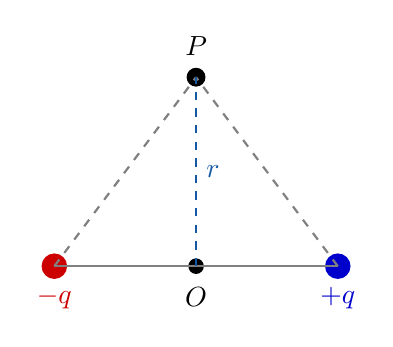
\begin{tikzpicture}[>=Stealth, thick, scale=1.2]
        % Charges
        \filldraw [red!80!black] (-1.5,0) circle (3.5pt) node[below=4pt] {$-q$};
        \filldraw [blue!80!black] (1.5,0) circle (3.5pt) node[below=4pt] {$+q$};
        \filldraw [black] (0,0) circle (2pt) node[below=4pt] {$O$};
        \draw [thick, gray] (-1.5,0) -- (1.5,0);
        
        % Point P
        \filldraw [black] (0,2) circle (2.5pt) node[above=4pt] {$P$};
        \draw [dashed, gray] (-1.5,0) -- (0,2);
        \draw [dashed, gray] (1.5,0) -- (0,2);
        \draw [dashed, RoyalBlue] (0,0) -- (0,2) node[midway, right] {$r$};
    \end{tikzpicture}
\end{center}

\subsubsection*{Step 1}
Distance of \( P \) from each charge:
\[ r = \sqrt{x^2+a^2} \]
Field due to each charge:
\[ E = \frac{1}{4\pi\epsilon_0} \frac{q}{r^2} \]

\subsubsection*{Step 2}
Resolve into components. Vertical components cancel. Horizontal components add.

\subsubsection*{Step 3}
Net Field after simplification:
\[ E = \frac{1}{4\pi\epsilon_0} \frac{2qa}{r^3} \]
Using \( p = 2aq \),
\begin{tcolorbox}[colback=RoyalBlue!5!white, colframe=RoyalBlue]
    \[ E_{\text{equatorial}} = \frac{1}{4\pi\epsilon_0} \frac{p}{r^3} \]
\end{tcolorbox}

\subsubsection*{Final Result (Equatorial)}
\begin{tcolorbox}[colback=RoyalBlue!5!white, colframe=RoyalBlue]
    \[ E_{\text{equatorial}} = \frac{1}{4\pi\epsilon_0} \frac{p}{r^3} \]
\end{tcolorbox}

\subsection*{Comparison}
\begin{table}[htbp]
    \centering
    \caption{Electric Field Comparison}
    \vspace{0.2cm}
    \begin{tabular}{cc}
        \toprule
        \textbf{Position} & \textbf{Electric Field} \\
        \midrule
        Axial & \( \frac{1}{4\pi\epsilon_0}\frac{2p}{r^3} \) \\
        Equatorial & \( \frac{1}{4\pi\epsilon_0}\frac{p}{r^3} \) \\
        \bottomrule
    \end{tabular}
\end{table}

% ---

% =========================================================================
% DERIVATION 5
% =========================================================================
\section{Derivation 5: Biot--Savart Law}

\subsection*{PYQ Weightage}
\begin{tcolorbox}[colback=yellow!10!white, colframe=orange, halign=center]
    \textbf{PYQ Weightage: \textasteriskcentered\textasteriskcentered\textasteriskcentered\textasteriskcentered\textasteriskcentered\ Direct PYQ (Set 1, Set 2, Set 3)}
\end{tcolorbox}

\subsection*{Question}
State and derive Biot--Savart Law.

\subsection*{Statement}
The magnetic field at a point due to a small current element is:
\begin{enumerate}
    \item Directly proportional to current (\( I \))
    \item Directly proportional to current element (\( dl \))
    \item Directly proportional to \( \sin\theta \)
    \item Inversely proportional to square of distance (\( r^2 \))
\end{enumerate}

\subsection*{Diagram}
\begin{center}
    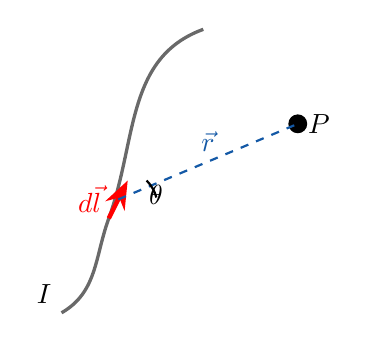
\begin{tikzpicture}[>=Stealth, thick, scale=1.2]
        % Wire
        \draw [very thick, dimgray] (-0.5,-1) to [out=30, in=250] (0,0) to [out=70, in=200] (1,2);
        \node [left] at (-0.5,-0.8) {$I$};
        
        % dl element
        \draw [->, red, ultra thick] (0,0) -- (0.2,0.4) node[midway, left=2pt] {$d\vec{l}$};
        
        % Point P
        \filldraw [black] (2,1) circle (2.5pt) node[right] {$P$};
        \draw [dashed, RoyalBlue] (0.1,0.2) -- (2,1) node[midway, above] {$\vec{r}$};
        
        % Angle theta
        \draw (0.4,0.4) arc (45:15:0.4);
        \node at (0.5,0.25) {$\theta$};
    \end{tikzpicture}
\end{center}

\subsection*{Experimental Observations}
Magnetic field (\( dB \)) is:
\begin{itemize}
    \item Directly proportional to current:
    \[ dB \propto I \]
    \item Directly proportional to current element:
    \[ dB \propto dl \]
    \item Directly proportional to \( \sin\theta \):
    \[ dB \propto \sin\theta \]
    \item Inversely proportional to square of distance:
    \[ dB \propto \frac{1}{r^2} \]
\end{itemize}

Combining all:
\[ dB \propto \frac{I \, dl \sin\theta}{r^2} \]

Introducing proportionality constant \( \frac{\mu_0}{4\pi} \), hence
\begin{tcolorbox}[colback=RoyalBlue!5!white, colframe=RoyalBlue]
    \[ dB = \frac{\mu_0}{4\pi} \frac{I \, dl \sin\theta}{r^2} \]
\end{tcolorbox}

\subsection*{Vector Form}
\begin{tcolorbox}[colback=RoyalBlue!5!white, colframe=RoyalBlue]
    \[ d\vec{B} = \frac{\mu_0}{4\pi} \frac{I(d\vec{l} \times \hat{r})}{r^2} \]
\end{tcolorbox}

\subsection*{Special Cases}
\begin{itemize}
    \item \textbf{Case 1: \( \theta = 0^\circ \)}
    \[ \sin0^\circ = 0 \]
    \begin{tcolorbox}[colback=RoyalBlue!5!white, colframe=RoyalBlue]
        \[ dB = 0 \]
    \end{tcolorbox}
    \item \textbf{Case 2: \( \theta = 90^\circ \)}
    \[ \sin90^\circ = 1 \]
    \begin{tcolorbox}[colback=RoyalBlue!5!white, colframe=RoyalBlue]
        \[ dB = \frac{\mu_0}{4\pi} \frac{I \, dl}{r^2} \]
    \end{tcolorbox}
    Maximum magnetic field.
\end{itemize}

\subsection*{Final Result}
\begin{tcolorbox}[colback=RoyalBlue!5!white, colframe=RoyalBlue]
    \[ dB = \frac{\mu_0}{4\pi} \frac{I \, dl \sin\theta}{r^2} \]
\end{tcolorbox}

\subsection*{Exam Ending Line}
Hence proved the Biot--Savart law for magnetic field due to a current element.

\newpage

% =========================================================================
% DERIVATION 6
% =========================================================================
\section{Derivation 6: Magnetic Field Due to Infinite Straight Wire}

\subsection*{PYQ Weightage}
\begin{tcolorbox}[colback=yellow!10!white, colframe=orange, halign=center]
    \textbf{PYQ Weightage: \textasteriskcentered\textasteriskcentered\textasteriskcentered\textasteriskcentered\textasteriskcentered\ Direct PYQ}
\end{tcolorbox}

\subsection*{Question}
Using Biot--Savart law, obtain an expression for magnetic field due to an infinitely long straight current-carrying conductor.

\subsection*{Diagram}
\begin{center}
    \begin{tikzpicture}[>=Stealth, thick, scale=1.2]
        % Vertical Wire
        \draw [very thick, red] (0,-2.5) -- (0,2.5) node[above] {$I$};
        
        % Point P
        \filldraw [black] (2,0) circle (2.5pt) node[right] {$P$};
        \draw [dashed, gray] (0,0) -- (2,0) node[midway, above] {$x$};
        
        % Line element dl at y
        \filldraw [RoyalBlue] (0,1.2) circle (2pt) node[left] {$dl$};
        \draw [dashed, RoyalBlue] (0,1.2) -- (2,0) node[midway, above right] {$r$};
        
        % Angle theta
        \draw (0,0.9) arc (270:320:0.3);
        \node at (0.2,0.8) {$\theta$};
    \end{tikzpicture}
\end{center}

\subsection*{Step 1}
From Biot--Savart Law,
\[ dB = \frac{\mu_0}{4\pi} \frac{I \, dl \sin\theta}{r^2} \]

\subsection*{Step 2}
From geometry,
\[ r = x \csc\theta \]
and
\[ dl = x \csc^2\theta \, d\theta \]

\subsection*{Step 3}
Substitute in Biot--Savart law:
\[ dB = \frac{\mu_0 I}{4\pi} \frac{x \csc^2\theta \sin\theta \, d\theta}{x^2 \csc^2\theta} \]
Simplifying,
\[ dB = \frac{\mu_0 I}{4\pi x} \sin\theta \, d\theta \]

\subsection*{Step 4}
Integrate for infinite wire:
\( \theta = -90^\circ \) to \( \theta = +90^\circ \).
Thus
\[ B = \frac{\mu_0 I}{4\pi x} \int_{-\pi/2}^{+\pi/2} \sin\theta \, d\theta \]

\subsection*{Step 5}
\[ B = \frac{\mu_0 I}{4\pi x} \left[ -\cos\theta \right]_{-\pi/2}^{+\pi/2} \]
\[ B = \frac{\mu_0 I}{4\pi x} (2) \]
Therefore
\begin{tcolorbox}[colback=RoyalBlue!5!white, colframe=RoyalBlue]
    \[ B = \frac{\mu_0 I}{2\pi x} \]
\end{tcolorbox}

\subsection*{Final Result}
\begin{tcolorbox}[colback=RoyalBlue!5!white, colframe=RoyalBlue]
    \[ B = \frac{\mu_0 I}{2\pi r} \]
\end{tcolorbox}

\subsection*{Exam Ending Line}
Hence the magnetic field due to an infinitely long straight conductor varies inversely with distance from the conductor.

\newpage

% =========================================================================
% DERIVATION 7
% =========================================================================
\section{Derivation 7: Magnetic Field on Axis of Circular Coil}

\subsection*{PYQ Weightage}
\begin{tcolorbox}[colback=yellow!10!white, colframe=orange, halign=center]
    \textbf{PYQ Weightage: \textasteriskcentered\textasteriskcentered\textasteriskcentered\textasteriskcentered\textasteriskcentered\ Direct 10-Mark PYQ (Set 1)}
\end{tcolorbox}

\subsection*{Question}
Derive an expression for magnetic field at a point on the axis of a circular current-carrying coil.

\subsection*{Diagram}
\begin{center}
    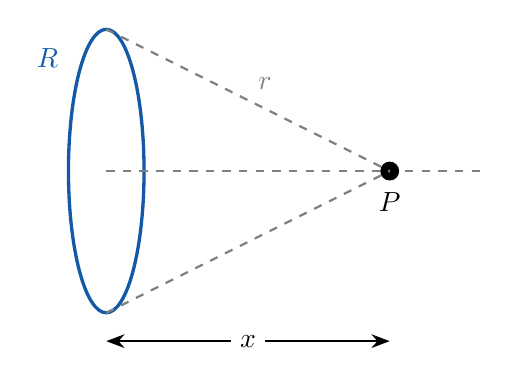
\begin{tikzpicture}[>=Stealth, thick, scale=1.2]
        % Ellipse for loop
        \draw[very thick, RoyalBlue] (0,0) ellipse (0.4 and 1.5);
        \node[left, RoyalBlue] at (-0.4, 1.2) {$R$};
        
        % Axis line
        \draw[dashed, gray] (0,0) -- (4,0);
        
        % Point P on axis
        \filldraw [black] (3,0) circle (2.5pt) node[below=4pt] {$P$};
        \draw[<->] (0,-1.8) -- (3,-1.8) node[midway, fill=white] {$x$};
        
        % Lines from top/bottom of coil to P
        \draw[dashed, gray] (0,1.5) -- (3,0) node[midway, above right] {$r$};
        \draw[dashed, gray] (0,-1.5) -- (3,0);
    \end{tikzpicture}
\end{center}

\subsection*{Step 1}
Consider a small current element (\( dl \)). Using Biot--Savart Law,
\[ dB = \frac{\mu_0}{4\pi} \frac{I \, dl}{r^2} \]
because \( \theta = 90^\circ \).

\subsection*{Step 2}
Distance of point (\( P \)) from every element:
\begin{tcolorbox}[colback=RoyalBlue!5!white, colframe=RoyalBlue]
    \[ r = \sqrt{R^2+x^2} \]
\end{tcolorbox}

\subsection*{Step 3}
Resolve (\( dB \)) into components. Due to symmetry, perpendicular components cancel while axial components add.
Hence
\[ dB_x = dB \cos\phi \]

\subsection*{Step 4}
Substitute:
\[ dB_x = \frac{\mu_0}{4\pi} \frac{I \, dl}{r^2} \cos\phi \]
From geometry,
\[ \cos\phi = \frac{R}{r} \]
Therefore
\[ dB_x = \frac{\mu_0}{4\pi} \frac{I R \, dl}{r^3} \]

\subsection*{Step 5}
Integrate around complete coil:
\[ B = \frac{\mu_0 I R}{4\pi r^3} \oint dl \]
But
\[ \oint dl = 2\pi R \]
Hence
\[ B = \frac{\mu_0 I R}{4\pi r^3} (2\pi R) \]
\[ B = \frac{\mu_0 I R^2}{2r^3} \]
Substitute \( r = \sqrt{R^2+x^2} \).

\subsection*{Final Result}
\begin{tcolorbox}[colback=RoyalBlue!5!white, colframe=RoyalBlue]
    \[ B = \frac{\mu_0 I R^2}{2(R^2+x^2)^{3/2}} \]
\end{tcolorbox}

\subsubsection*{For N Turns Coil}
\begin{tcolorbox}[colback=RoyalBlue!5!white, colframe=RoyalBlue]
    \[ B = \frac{\mu_0 N I R^2}{2(R^2+x^2)^{3/2}} \]
\end{tcolorbox}

\subsubsection*{At Centre (\( x = 0 \))}
\begin{tcolorbox}[colback=RoyalBlue!5!white, colframe=RoyalBlue]
    \[ B = \frac{\mu_0 N I}{2R} \]
\end{tcolorbox}

% ---

% =========================================================================
% DERIVATION 8
% =========================================================================
\section{Derivation 8: Ampere's Circuital Law}

\subsection*{PYQ Weightage}
\begin{tcolorbox}[colback=yellow!10!white, colframe=orange, halign=center]
    \textbf{PYQ Weightage: \textasteriskcentered\textasteriskcentered\textasteriskcentered\textasteriskcentered\textasteriskcentered\ Important Derivation}
\end{tcolorbox}

\subsection*{Question}
State and explain Ampere's Circuital Law.

\subsection*{Statement}
The line integral of magnetic field around any closed path is equal to \( \mu_0 \) times the net current enclosed by the path.

\subsection*{Diagram}
\begin{center}
    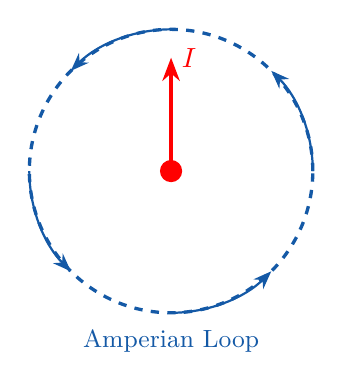
\begin{tikzpicture}[>=Stealth, thick, scale=1.2]
        % Circular Amperian loop
        \draw [dashed, RoyalBlue, very thick] (0,0) circle (1.5);
        \node [RoyalBlue] at (0,-1.8) {\small Amperian Loop};
        
        % Current in middle
        \filldraw [red] (0,0) circle (3pt);
        \draw [->, red, very thick] (0,0) -- (0,1.2) node[right] {$I$};
        
        % Arrows for integration path direction
        \draw [->, RoyalBlue] (1.5,0) arc (0:45:1.5);
        \draw [->, RoyalBlue] (0,1.5) arc (90:135:1.5);
        \draw [->, RoyalBlue] (-1.5,0) arc (180:225:1.5);
        \draw [->, RoyalBlue] (0,-1.5) arc (270:315:1.5);
    \end{tikzpicture}
\end{center}

\subsection*{Mathematical Form}
\begin{tcolorbox}[colback=RoyalBlue!5!white, colframe=RoyalBlue]
    \[ \oint \vec{B} \cdot d\vec{l} = \mu_0 I_{\text{enc}} \]
\end{tcolorbox}

\subsection*{Explanation}
Consider a current carrying conductor enclosed by a circular path. Magnetic field at every point on the circular path is constant.
Also
\[ \vec{B} \parallel d\vec{l} \]
Therefore
\[ \vec{B} \cdot d\vec{l} = B \, dl \]
Hence
\[ \oint \vec{B} \cdot d\vec{l} = B \oint dl \]
Since total enclosed current is \( I \),
\begin{tcolorbox}[colback=RoyalBlue!5!white, colframe=RoyalBlue]
    \[ \oint \vec{B} \cdot d\vec{l} = \mu_0 I \]
\end{tcolorbox}

\subsection*{Final Result}
\begin{tcolorbox}[colback=RoyalBlue!5!white, colframe=RoyalBlue]
    \[ \oint \vec{B} \cdot d\vec{l} = \mu_0 I \]
\end{tcolorbox}

\subsection*{Exam Ending Line}
Hence proved Ampere's Circuital Law.

\newpage

% =========================================================================
% DERIVATION 9
% =========================================================================
\section{Derivation 9: Magnetic Field Inside a Long Solenoid}

\subsection*{PYQ Weightage}
\begin{tcolorbox}[colback=yellow!10!white, colframe=orange, halign=center]
    \textbf{PYQ Weightage: \textasteriskcentered\textasteriskcentered\textasteriskcentered\textasteriskcentered\textasteriskcentered\ Direct PYQ}
\end{tcolorbox}

\subsection*{Question}
Using Ampere's Circuital Law, obtain an expression for magnetic field inside a long solenoid.

\subsection*{Diagram}
\begin{center}
    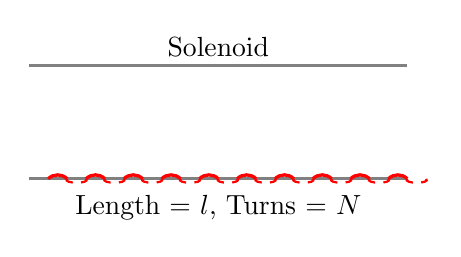
\begin{tikzpicture}[>=Stealth, thick, scale=1.2]
        % Solenoid representation
        \draw[very thick, gray] (0,0.6) -- (4,0.6);
        \draw[very thick, gray] (0,-0.6) -- (4,-0.6);
        \foreach \x in {0.2, 0.6, 1.0, 1.4, 1.8, 2.2, 2.6, 3.0, 3.4, 3.8} {
            \draw[red, very thick] (\x,-0.6) to[out=45, in=135] (\x+0.2,-0.6);
            \draw[red, dashed] (\x+0.2,-0.6) to[out=225, in=315] (\x+0.4,-0.6);
        }
        \node at (2,0.8) {Solenoid};
        \node at (2,-0.9) {Length = $l$, Turns = $N$};
    \end{tikzpicture}
\end{center}

\subsection*{Step 1}
Choose rectangular Amperian loop.
\begin{center}
    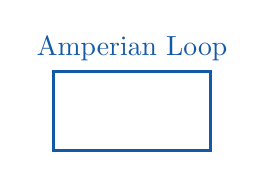
\begin{tikzpicture}[>=Stealth, thick]
        % Amperian loop rectangle
        \draw[RoyalBlue, very thick] (0.5, -0.4) rectangle (2.5, 0.6);
        \node[above, RoyalBlue] at (1.5, 0.6) {Amperian Loop};
    \end{tikzpicture}
\end{center}

\subsection*{Step 2: Apply Ampere's Law}
\[ \oint \vec{B} \cdot d\vec{l} = \mu_0 I_{\text{enc}} \]

\subsection*{Step 3}
Outside solenoid:
\[ B \approx 0 \]
Hence only inside path contributes.
\[ Bl = \mu_0 I_{\text{enc}} \]

\subsection*{Step 4}
Turns per unit length:
\[ n = \frac{N}{l} \]
Number of turns enclosed: \( nl \).
Current enclosed:
\[ I_{\text{enc}} = nlI \]

\subsection*{Step 5}
Substitute:
\[ Bl = \mu_0(nlI) \]
Cancel \( l \):
\begin{tcolorbox}[colback=RoyalBlue!5!white, colframe=RoyalBlue]
    \[ B = \mu_0 nI \]
\end{tcolorbox}

\subsection*{Final Result}
\begin{tcolorbox}[colback=RoyalBlue!5!white, colframe=RoyalBlue]
    \[ B = \mu_0 nI \]
\end{tcolorbox}

\subsubsection*{Solenoid With Core}
\begin{tcolorbox}[colback=RoyalBlue!5!white, colframe=RoyalBlue]
    \[ B = \mu_0 \mu_r nI \]
\end{tcolorbox}

\subsection*{Exam Ending Line}
Hence magnetic field inside a long solenoid is uniform and equals
\begin{tcolorbox}[colback=RoyalBlue!5!white, colframe=RoyalBlue]
    \[ B = \mu_0 nI \]
\end{tcolorbox}

\newpage

% =========================================================================
% DERIVATION 10
% =========================================================================
\section{Derivation 10: Relation Between Permeability and Susceptibility}

\subsection*{PYQ Weightage}
\begin{tcolorbox}[colback=yellow!10!white, colframe=orange, halign=center]
    \textbf{PYQ Weightage: \textasteriskcentered\textasteriskcentered\textasteriskcentered\textasteriskcentered\ Direct PYQ}
\end{tcolorbox}

\subsection*{Question}
Prove that
\[ \mu = \mu_0(1+\chi) \]

\subsection*{Step 1}
Magnetic induction in a material:
\[ B = \mu_0(H+M) \]

\subsection*{Step 2}
Using \( M = \chi H \), substitute:
\[ B = \mu_0(H+\chi H) \]
\[ B = \mu_0 H(1+\chi) \]

\subsection*{Step 3}
But \( B = \mu H \), therefore
\[ \mu H = \mu_0 H(1+\chi) \]
Cancel \( H \):
\begin{tcolorbox}[colback=RoyalBlue!5!white, colframe=RoyalBlue]
    \[ \mu = \mu_0(1+\chi) \]
\end{tcolorbox}

\subsection*{Final Result}
\begin{tcolorbox}[colback=RoyalBlue!5!white, colframe=RoyalBlue]
    \[ \mu = \mu_0(1+\chi) \]
\end{tcolorbox}

\subsubsection*{Also}
\begin{tcolorbox}[colback=RoyalBlue!5!white, colframe=RoyalBlue]
    \[ \mu_r = 1+\chi \]
\end{tcolorbox}

\newpage

% =========================================================================
% DERIVATION 11
% =========================================================================
\section{Derivation 11: Faraday's Second Law}

\subsection*{PYQ Weightage}
\begin{tcolorbox}[colback=yellow!10!white, colframe=orange, halign=center]
    \textbf{PYQ Weightage: \textasteriskcentered\textasteriskcentered\textasteriskcentered\textasteriskcentered\textasteriskcentered\ Direct PYQ}
\end{tcolorbox}

\subsection*{Question}
State and derive Faraday's Second Law of Electromagnetic Induction.

\subsection*{Statement}
The induced emf is equal to the negative rate of change of magnetic flux linked with the circuit.

\subsection*{Diagram}
\begin{center}
    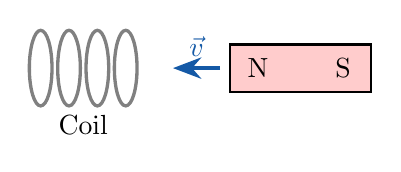
\begin{tikzpicture}[>=Stealth, thick, scale=1.2]
        % Coil representation
        \foreach \x in {0, 0.3, 0.6, 0.9} {
            \draw[very thick, gray] (\x, 0) ellipse (0.12 and 0.4);
        }
        \node at (0.45, -0.6) {Coil};
        
        % Magnet
        \draw[fill=red!20] (2, -0.25) rectangle (3.5, 0.25);
        \node at (2.3, 0) {N};
        \node at (3.2, 0) {S};
        \draw[->, ultra thick, RoyalBlue] (1.9, 0) -- (1.4, 0) node[midway, above] {$\vec{v}$};
    \end{tikzpicture}
\end{center}

\subsection*{Step 1}
Let magnetic flux change from \( \phi_1 \) to \( \phi_2 \) in time \( \Delta t \).

\subsection*{Step 2}
Experimentally,
\[ e \propto \frac{\Delta\phi}{\Delta t} \]

\subsection*{Step 3}
Introducing negative sign according to Lenz's Law,
\[ e = -\frac{\Delta\phi}{\Delta t} \]
For infinitesimal changes,
\begin{tcolorbox}[colback=RoyalBlue!5!white, colframe=RoyalBlue]
    \[ e = -\frac{d\phi}{dt} \]
\end{tcolorbox}

\subsubsection*{For N Turns Coil}
\begin{tcolorbox}[colback=RoyalBlue!5!white, colframe=RoyalBlue]
    \[ e = -N\frac{d\phi}{dt} \]
\end{tcolorbox}

\subsection*{Final Result}
\begin{tcolorbox}[colback=RoyalBlue!5!white, colframe=RoyalBlue]
    \[ e = -N\frac{d\phi}{dt} \]
\end{tcolorbox}

\newpage

% =========================================================================
% DERIVATION 12
% =========================================================================
\section{Derivation 12: Self-Inductance of a Long Solenoid}

\subsection*{PYQ Weightage}
\begin{tcolorbox}[colback=yellow!10!white, colframe=orange, halign=center]
    \textbf{PYQ Weightage: \textasteriskcentered\textasteriskcentered\textasteriskcentered\textasteriskcentered\textasteriskcentered\ Direct PYQ}
\end{tcolorbox}

\subsection*{Question}
Derive an expression for self-inductance of a long solenoid.

\subsection*{Diagram}
\begin{center}
    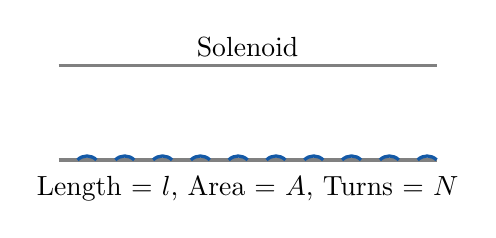
\begin{tikzpicture}[>=Stealth, thick, scale=1.2]
        % Solenoid
        \draw[very thick, gray] (0,0.5) -- (4,0.5);
        \draw[very thick, gray] (0,-0.5) -- (4,-0.5);
        \foreach \x in {0.2, 0.6, 1.0, 1.4, 1.8, 2.2, 2.6, 3.0, 3.4, 3.8} {
            \draw[RoyalBlue, very thick] (\x,-0.5) to[out=45, in=135] (\x+0.2,-0.5);
        }
        \node at (2,0.7) {Solenoid};
        \node at (2,-0.8) {Length = $l$, Area = $A$, Turns = $N$};
    \end{tikzpicture}
\end{center}

\subsection*{Step 1}
Magnetic field inside solenoid:
\[ B = \mu_0 n I \]
where \( n = \frac{N}{l} \).
Hence
\[ B = \mu_0 \frac{N}{l} I \]

\subsection*{Step 2}
Magnetic flux through one turn:
\[ \phi = BA \]
Substituting,
\[ \phi = \mu_0 \frac{N}{l} I A \]

\subsection*{Step 3}
Flux linkage:
\[ N\phi = N \left( \mu_0 \frac{N}{l} I A \right) \]
\[ N\phi = \mu_0 \frac{N^2 A}{l} I \]

\subsection*{Step 4}
Using \( L = \frac{N\phi}{I} \), therefore
\begin{tcolorbox}[colback=RoyalBlue!5!white, colframe=RoyalBlue]
    \[ L = \frac{\mu_0 N^2 A}{l} \]
\end{tcolorbox}

\subsection*{Final Result}
\begin{tcolorbox}[colback=RoyalBlue!5!white, colframe=RoyalBlue]
    \[ L = \frac{\mu_0 N^2 A}{l} \]
\end{tcolorbox}

% ---

% =========================================================================
% DERIVATION 13
% =========================================================================
\section{Derivation 13: Continuity Equation}

\subsection*{PYQ Weightage}
\begin{tcolorbox}[colback=yellow!10!white, colframe=orange, halign=center]
    \textbf{PYQ Weightage: \textasteriskcentered\textasteriskcentered\textasteriskcentered\textasteriskcentered\textasteriskcentered\ Direct PYQ (Set 2)}
\end{tcolorbox}

\subsection*{Question}
Derive the Continuity Equation and explain its physical significance.

\subsection*{Statement}
The continuity equation expresses the law of conservation of electric charge.

\subsection*{Diagram}
\begin{center}
    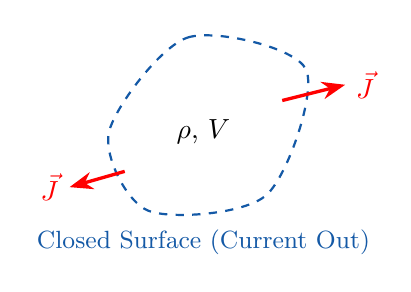
\begin{tikzpicture}[>=Stealth, thick]
        % Closed volume
        \draw [dashed, RoyalBlue] plot [smooth cycle] coordinates {(0,0) (1,1.2) (2.5,0.8) (2,-0.8) (0.5,-1)};
        \node at (1.2,0) {$\rho$, $V$};
        % Arrows pointing outward
        \draw [->, red, very thick] (2.2,0.4) -- (3,0.6) node[right] {$\vec{J}$};
        \draw [->, red, very thick] (0.2,-0.5) -- (-0.5,-0.7) node[left] {$\vec{J}$};
        \node [RoyalBlue] at (1.2,-1.4) {\small Closed Surface (Current Out)};
    \end{tikzpicture}
\end{center}

\subsection*{Step 1: Charge Inside Volume}
Let charge density inside volume \( V \) be \( \rho \).
Total charge inside volume:
\[ Q = \int \rho \, dV \]

\subsection*{Step 2: Current Leaving Surface}
Current density: \( \vec{J} \).
Total current flowing out:
\[ I = \oint \vec{J} \cdot d\vec{S} \]

\subsection*{Step 3: Conservation of Charge}
Rate of decrease of charge inside volume equals current flowing out.
\begin{tcolorbox}[colback=RoyalBlue!5!white, colframe=RoyalBlue]
    \[ \oint \vec{J} \cdot d\vec{S} = -\frac{d}{dt} \int \rho \, dV \]
\end{tcolorbox}

\subsection*{Step 4: Apply Divergence Theorem}
\[ \oint \vec{J} \cdot d\vec{S} = \int (\nabla \cdot \vec{J}) \, dV \]
Substituting,
\[ \int (\nabla \cdot \vec{J}) \, dV = -\int \frac{\partial\rho}{\partial t} \, dV \]

\subsection*{Step 5: Equate Integrands}
Since equation is valid for every volume,
\[ \nabla \cdot \vec{J} = -\frac{\partial\rho}{\partial t} \]
Therefore
\begin{tcolorbox}[colback=RoyalBlue!5!white, colframe=RoyalBlue]
    \[ \nabla \cdot \vec{J} + \frac{\partial\rho}{\partial t} = 0 \]
\end{tcolorbox}

\subsection*{Final Result}
\begin{tcolorbox}[colback=RoyalBlue!5!white, colframe=RoyalBlue]
    \[ \nabla \cdot \vec{J} + \frac{\partial\rho}{\partial t} = 0 \]
\end{tcolorbox}

\subsection*{Physical Significance}
Represents:
\begin{tcolorbox}[colback=RoyalBlue!5!white, colframe=RoyalBlue]
    \[ \text{Conservation of Charge} \]
\end{tcolorbox}
Charge can neither be created nor destroyed.

\subsection*{Exam Ending Line}
Hence proved the continuity equation.

\newpage

% =========================================================================
% DERIVATION 14
% =========================================================================
\section{Derivation 14: Maxwell's Equations}

\subsection*{PYQ Weightage}
\begin{tcolorbox}[colback=yellow!10!white, colframe=orange, halign=center]
    \textbf{PYQ Weightage: \textasteriskcentered\textasteriskcentered\textasteriskcentered\textasteriskcentered\textasteriskcentered\ Direct 10-Mark PYQ}
\end{tcolorbox}

\subsection*{Question}
Write Maxwell's equations in integral and differential forms and explain their significance.

\subsection*{Maxwell's First Equation: Gauss's Law for Electricity}

\subsubsection*{Integral Form}
\begin{tcolorbox}[colback=RoyalBlue!5!white, colframe=RoyalBlue]
    \[ \oint \vec{E} \cdot d\vec{S} = \frac{Q}{\epsilon_0} \]
\end{tcolorbox}

\subsubsection*{Differential Form}
\begin{tcolorbox}[colback=RoyalBlue!5!white, colframe=RoyalBlue]
    \[ \nabla \cdot \vec{E} = \frac{\rho}{\epsilon_0} \]
\end{tcolorbox}

\subsubsection*{Physical Meaning}
Electric charges are sources of electric field.

\subsubsection*{Diagram}
\begin{center}
    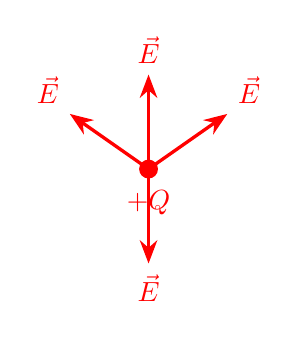
\begin{tikzpicture}[>=Stealth, thick]
        \filldraw [red] (0,0) circle (3pt) node[below=4pt] {$+Q$};
        \draw [->, red, very thick] (0,0) -- (0,1.2) node[above] {$\vec{E}$};
        \draw [->, red, very thick] (0,0) -- (1,0.7) node[above right] {$\vec{E}$};
        \draw [->, red, very thick] (0,0) -- (-1,0.7) node[above left] {$\vec{E}$};
        \draw [->, red, very thick] (0,0) -- (0,-1.2) node[below] {$\vec{E}$};
    \end{tikzpicture}
\end{center}

\subsection*{Maxwell's Second Equation: Gauss's Law for Magnetism}

\subsubsection*{Integral Form}
\begin{tcolorbox}[colback=RoyalBlue!5!white, colframe=RoyalBlue]
    \[ \oint \vec{B} \cdot d\vec{S} = 0 \]
\end{tcolorbox}

\subsubsection*{Differential Form}
\begin{tcolorbox}[colback=RoyalBlue!5!white, colframe=RoyalBlue]
    \[ \nabla \cdot \vec{B} = 0 \]
\end{tcolorbox}

\subsubsection*{Physical Meaning}
Magnetic monopoles do not exist.

\subsubsection*{Diagram}
\begin{center}
    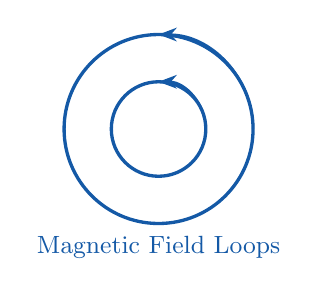
\begin{tikzpicture}[>=Stealth, thick]
        % Closed magnetic field loops
        \draw [RoyalBlue, very thick] (0,0) circle (0.6);
        \draw [RoyalBlue, very thick] (0,0) circle (1.2);
        \draw [->, RoyalBlue] (0.6,0) arc (0:90:0.6);
        \draw [->, RoyalBlue] (1.2,0) arc (0:90:1.2);
        \node [RoyalBlue] at (0,-1.5) {\small Magnetic Field Loops};
    \end{tikzpicture}
\end{center}

\subsection*{Maxwell's Third Equation: Faraday's Law}

\subsubsection*{Integral Form}
\begin{tcolorbox}[colback=RoyalBlue!5!white, colframe=RoyalBlue]
    \[ \oint \vec{E} \cdot d\vec{l} = -\frac{d\phi_B}{dt} \]
\end{tcolorbox}

\subsubsection*{Differential Form}
\begin{tcolorbox}[colback=RoyalBlue!5!white, colframe=RoyalBlue]
    \[ \nabla \times \vec{E} = -\frac{\partial\vec{B}}{\partial t} \]
\end{tcolorbox}

\subsubsection*{Physical Meaning}
Changing magnetic field produces electric field.

\subsubsection*{Diagram}
\begin{center}
    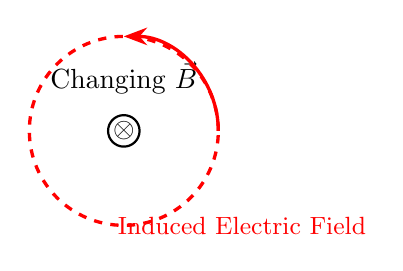
\begin{tikzpicture}[>=Stealth, thick]
        % Indicated changing B field
        \draw (0,0) circle (0.2) node {$\otimes$};
        \node [above=4pt] at (0,0.2) {Changing $\vec{B}$};
        % Induced electric field loop
        \draw [dashed, red, very thick] (0,0) circle (1.2);
        \draw [->, red, very thick] (1.2,0) arc (0:90:1.2);
        \node [red] at (1.5,-1.2) {\small Induced Electric Field};
    \end{tikzpicture}
\end{center}

\subsection*{Maxwell's Fourth Equation: Ampere-Maxwell Law}

\subsubsection*{Integral Form}
\begin{tcolorbox}[colback=RoyalBlue!5!white, colframe=RoyalBlue]
    \[ \oint \vec{B} \cdot d\vec{l} = \mu_0 I + \mu_0\epsilon_0\frac{d\phi_E}{dt} \]
\end{tcolorbox}

\subsubsection*{Differential Form}
\begin{tcolorbox}[colback=RoyalBlue!5!white, colframe=RoyalBlue]
    \[ \nabla \times \vec{B} = \mu_0\vec{J} + \mu_0\epsilon_0\frac{\partial\vec{E}}{\partial t} \]
\end{tcolorbox}

\subsubsection*{Physical Meaning}
Magnetic field is produced by:
\begin{enumerate}
    \item Conduction current
    \item Changing electric field
\end{enumerate}

\subsubsection*{Diagram}
\begin{center}
    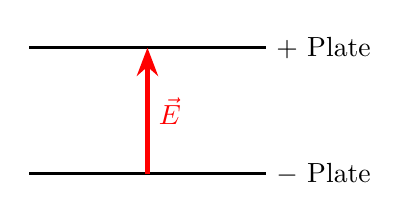
\begin{tikzpicture}[>=Stealth, thick]
        % Capacitor plates
        \draw [very thick] (-1.5,0.8) -- (1.5,0.8) node[right] {$+$ Plate};
        \draw [very thick] (-1.5,-0.8) -- (1.5,-0.8) node[right] {$-$ Plate};
        % Field line
        \draw [->, red, ultra thick] (0,-0.8) -- (0,0.8) node[midway, right] {$\vec{E}$};
    \end{tikzpicture}
\end{center}

\subsection*{Maxwell Equation Summary Table}
\begin{table}[htbp]
    \centering
    \caption{Maxwell's Equations Summary}
    \vspace{0.2cm}
    \begin{tabular}{ll}
        \toprule
        \textbf{Equation} & \textbf{Differential Form} \\
        \midrule
        Gauss (Electric) & \( \nabla\cdot\vec{E}=\rho/\epsilon_0 \) \\
        Gauss (Magnetic) & \( \nabla\cdot\vec{B}=0 \) \\
        Faraday Law & \( \nabla\times\vec{E}=-\partial\vec{B}/\partial t \) \\
        Ampere-Maxwell Law & \( \nabla\times\vec{B}=\mu_0\vec{J}+\mu_0\epsilon_0\partial\vec{E}/\partial t \) \\
        \bottomrule
    \end{tabular}
\end{table}

\subsection*{Exam Ending Line}
Hence Maxwell unified electricity and magnetism into one theory.

\newpage

% =========================================================================
% DERIVATION 15
% =========================================================================
\section{Derivation 15: Thevenin's Theorem}

\subsection*{PYQ Weightage}
\begin{tcolorbox}[colback=yellow!10!white, colframe=orange, halign=center]
    \textbf{PYQ Weightage: \textasteriskcentered\textasteriskcentered\textasteriskcentered\textasteriskcentered\textasteriskcentered\ Direct PYQ}
\end{tcolorbox}

\subsection*{Question}
State and explain Thevenin's theorem.

\subsection*{Statement}
Any linear bilateral network can be replaced by an equivalent voltage source (\( V_{\text{th}} \)) in series with an equivalent resistance (\( R_{\text{th}} \)).

\subsection*{Original Circuit}
\begin{center}
    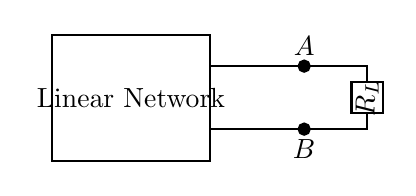
\begin{tikzpicture}[>=Stealth, thick]
        % Box representing network
        \draw (0,-0.8) rectangle (2,0.8) node[midway] {Linear Network};
        \draw (2,0.4) -- (3.2,0.4) node[above] {$A$};
        \draw (2,-0.4) -- (3.2,-0.4) node[below] {$B$};
        \filldraw (3.2,0.4) circle (2pt);
        \filldraw (3.2,-0.4) circle (2pt);
        % Load resistor RL
        \draw (3.2,0.4) -- (4,0.4) -- (4,0.2);
        \draw (3.8,-0.2) rectangle (4.2,0.2) node[midway, rotate=90] {$R_L$};
        \draw (4,-0.2) -- (4,-0.4) -- (3.2,-0.4);
    \end{tikzpicture}
\end{center}

\subsection*{Equivalent Circuit}
\begin{center}
    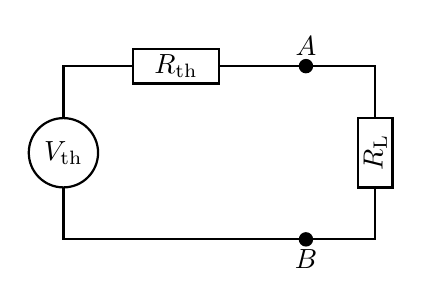
\begin{tikzpicture}[>=Stealth, thick, scale=1.1]
        % Circle for Vth
        \draw (0,0) circle (0.4cm) node {$V_{\text{th}}$};
        \draw (0,0.4) -- (0,1) -- (0.8,1);
        % Resistor Rth
        \draw (0.8,0.8) rectangle (1.8, 1.2) node[midway] {$R_{\text{th}}$};
        \draw (1.8,1) -- (2.8,1);
        % Terminal A
        \filldraw (2.8,1) circle (2pt) node[above] {$A$};
        \draw (2.8,1) -- (3.6,1) -- (3.6,0.4);
        % Resistor RL
        \draw (3.4,-0.4) rectangle (3.8, 0.4) node[midway, rotate=90] {$R_{\text{L}}$};
        \draw (3.6,-0.4) -- (3.6,-1) -- (2.8,-1);
        % Terminal B
        \filldraw (2.8,-1) circle (2pt) node[below] {$B$};
        \draw (2.8,-1) -- (0,-1) -- (0,-0.4);
    \end{tikzpicture}
\end{center}

\subsection*{Procedure}
\subsubsection*{Step 1}
Remove load resistor (\( R_L \)).

\subsubsection*{Step 2: Find open-circuit voltage}
\begin{tcolorbox}[colback=RoyalBlue!5!white, colframe=RoyalBlue]
    \[ V_{\text{th}} = V_{\text{OC}} \]
\end{tcolorbox}

\subsubsection*{Step 3: Deactivate sources}
\begin{itemize}
    \item Voltage source \(\rightarrow\) Short circuit
    \item Current source \(\rightarrow\) Open circuit
\end{itemize}

\subsubsection*{Step 4: Find equivalent resistance}
\begin{tcolorbox}[colback=RoyalBlue!5!white, colframe=RoyalBlue]
    \[ R_{\text{th}} \]
\end{tcolorbox}

\subsubsection*{Step 5: Reconnect load}

\subsubsection*{Load Current}
\begin{tcolorbox}[colback=RoyalBlue!5!white, colframe=RoyalBlue]
    \[ I = \frac{V_{\text{th}}}{R_{\text{th}}+R_L} \]
\end{tcolorbox}

\subsection*{Final Result}
Equivalent circuit becomes
\begin{tcolorbox}[colback=RoyalBlue!5!white, colframe=RoyalBlue]
    \[ V_{\text{th}} \text{ in series with } R_{\text{th}} \]
\end{tcolorbox}

\newpage

% =========================================================================
% DERIVATION 16
% =========================================================================
\section{Derivation 16: Maximum Power Transfer Theorem}

\subsection*{PYQ Weightage}
\begin{tcolorbox}[colback=yellow!10!white, colframe=orange, halign=center]
    \textbf{PYQ Weightage: \textasteriskcentered\textasteriskcentered\textasteriskcentered\textasteriskcentered\textasteriskcentered\ Direct PYQ}
\end{tcolorbox}

\subsection*{Question}
Prove that maximum power is transferred when load resistance equals source resistance.

\subsection*{Circuit}
\begin{center}
    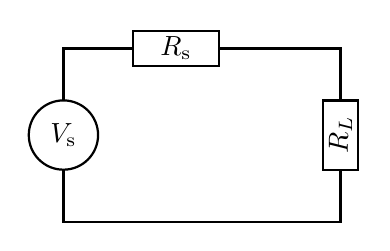
\begin{tikzpicture}[>=Stealth, thick, scale=1.1]
        % Voltage source Vs
        \draw (0,0) circle (0.4cm) node {$V_{\text{s}}$};
        \draw (0,0.4) -- (0,1) -- (0.8,1);
        % Resistor Rs
        \draw (0.8,0.8) rectangle (1.8, 1.2) node[midway] {$R_{\text{s}}$};
        \draw (1.8,1) -- (2.6,1);
        % Load resistor RL
        \draw (2.6,1) -- (3.2,1) -- (3.2,0.4);
        \draw (3.0,-0.4) rectangle (3.4, 0.4) node[midway, rotate=90] {$R_L$};
        \draw (3.2,-0.4) -- (3.2,-1) -- (0,-1) -- (0,-0.4);
    \end{tikzpicture}
\end{center}

\subsection*{Step 1: Current}
\[ I = \frac{V_s}{R_s+R_L} \]

\subsection*{Step 2: Load Power}
\[ P = I^2 R_L \]
Substituting current,
\[ P = \frac{V_s^2 R_L}{(R_s+R_L)^2} \]

\subsection*{Step 3: Differentiate}
For maximum power,
\[ \frac{dP}{dR_L} = 0 \]
Differentiating,
\[ (R_s+R_L) - 2R_L = 0 \]
\[ R_s - R_L = 0 \]
Therefore
\begin{tcolorbox}[colback=RoyalBlue!5!white, colframe=RoyalBlue]
    \[ R_L = R_s \]
\end{tcolorbox}

\subsection*{Condition for Maximum Power}
\begin{tcolorbox}[colback=RoyalBlue!5!white, colframe=RoyalBlue]
    \[ R_L = R_s \]
\end{tcolorbox}
or
\begin{tcolorbox}[colback=RoyalBlue!5!white, colframe=RoyalBlue]
    \[ R_L = R_{\text{th}} \]
\end{tcolorbox}

\subsection*{Step 4: Maximum Power}
Substitute \( R_L = R_s \):
\[ P_{\text{max}} = \frac{V_s^2}{4R_s} \]

\subsection*{Final Result}
\begin{tcolorbox}[colback=RoyalBlue!5!white, colframe=RoyalBlue]
    \[ P_{\text{max}} = \frac{V_s^2}{4R_s} \]
\end{tcolorbox}

\subsection*{Derivation Register Completed}
Most Important Exam Derivations:
\begin{itemize}
    \item[\checkmark] Gauss's Theorem
    \item[\checkmark] Electric Field due to Infinite Line Charge
    \item[\checkmark] Potential due to Dipole
    \item[\checkmark] Electric Field due to Dipole
    \item[\checkmark] Biot--Savart Law
    \item[\checkmark] Magnetic Field due to Infinite Straight Wire
    \item[\checkmark] Magnetic Field on Axis of Circular Coil
    \item[\checkmark] Ampere's Circuital Law
    \item[\checkmark] Magnetic Field Inside Solenoid
    \item[\checkmark] Relation \( \mu = \mu_0(1+\chi) \)
    \item[\checkmark] Faraday's Second Law
    \item[\checkmark] Self-Inductance of Solenoid
    \item[\checkmark] Continuity Equation
    \item[\checkmark] Maxwell's Equations
    \item[\checkmark] Thevenin's Theorem
    \item[\checkmark] Maximum Power Transfer Theorem
\end{itemize}
These are the derivations most strongly supported by your syllabus and repeated across Set 1, Set 2, and Set 3 PYQs.

\newpage

% =========================================================================
% DERIVATION 17
% =========================================================================
\section{Derivation 17: Mutual Inductance of Two Coaxial Solenoids}

\subsection*{PYQ Weightage}
\begin{tcolorbox}[colback=yellow!10!white, colframe=orange, halign=center]
    \textbf{PYQ Weightage: \textasteriskcentered\textasteriskcentered\textasteriskcentered\textasteriskcentered\textasteriskcentered\ Important Syllabus Derivation}
\end{tcolorbox}

\subsection*{Question}
Derive an expression for the mutual inductance of two long coaxial solenoids.

\subsection*{Diagram}
\begin{center}
    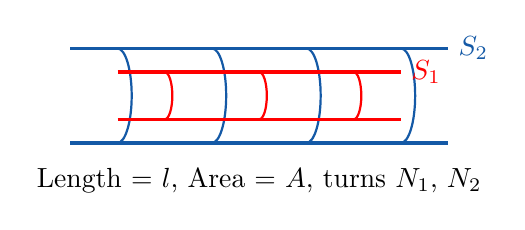
\begin{tikzpicture}[>=Stealth, thick, scale=1.2]
        % Outer Solenoid
        \draw[very thick, RoyalBlue] (0,0.5) -- (4,0.5);
        \draw[very thick, RoyalBlue] (0,-0.5) -- (4,-0.5);
        \foreach \x in {0.5, 1.5, 2.5, 3.5} {
            \draw[RoyalBlue] (\x,-0.5) arc (-90:90:0.15 and 0.5);
        }
        
        % Inner Solenoid
        \draw[very thick, red] (0.5,0.25) -- (3.5,0.25);
        \draw[very thick, red] (0.5,-0.25) -- (3.5,-0.25);
        \foreach \x in {1.0, 2.0, 3.0} {
            \draw[red] (\x,-0.25) arc (-90:90:0.08 and 0.25);
        }
        \node[right, RoyalBlue] at (4,0.5) {$S_2$};
        \node[right, red] at (3.5,0.25) {$S_1$};
        \node at (2,-0.9) {Length = $l$, Area = $A$, turns $N_1$, $N_2$};
    \end{tikzpicture}
\end{center}

\subsection*{Given}
Primary Solenoid:
\begin{itemize}
    \item \( N_1 \) turns
    \item Current: \( I_1 \)
\end{itemize}

Secondary Solenoid:
\begin{itemize}
    \item \( N_2 \) turns
\end{itemize}

Common parameters:
\begin{itemize}
    \item Common Area: \( A \)
    \item Length: \( l \)
\end{itemize}

\subsection*{Step 1: Magnetic Field Produced by Primary Solenoid}
Magnetic field inside long solenoid:
\[ B = \mu_0 n I \]
where \( n = \frac{N_1}{l} \).
Hence
\[ B = \mu_0 \frac{N_1}{l} I_1 \]

\subsection*{Step 2: Magnetic Flux Through One Turn of Secondary}
\[ \phi = BA \]
Substituting \( B \),
\[ \phi = \mu_0 \frac{N_1}{l} I_1 A \]

\subsection*{Step 3: Total Flux Linkage}
Flux linkage with secondary coil:
\[ N_2\phi = N_2 \left( \mu_0 \frac{N_1}{l} I_1 A \right) \]
\[ N_2\phi = \mu_0 \frac{N_1 N_2 A}{l} I_1 \]

\subsection*{Step 4: Definition of Mutual Inductance}
\begin{tcolorbox}[colback=RoyalBlue!5!white, colframe=RoyalBlue]
    \[ M = \frac{N_2\phi}{I_1} \]
\end{tcolorbox}
Substituting,
\[ M = \frac{\mu_0 \frac{N_1 N_2 A}{l} I_1}{I_1} \]
Cancelling \( I_1 \),
\begin{tcolorbox}[colback=RoyalBlue!5!white, colframe=RoyalBlue]
    \[ M = \frac{\mu_0 N_1 N_2 A}{l} \]
\end{tcolorbox}

\subsection*{Final Result}
\begin{tcolorbox}[colback=RoyalBlue!5!white, colframe=RoyalBlue]
    \[ M = \frac{\mu_0 N_1 N_2 A}{l} \]
\end{tcolorbox}

\subsection*{Important Observations}
\[ M \propto N_1 \]
\[ M \propto N_2 \]
\[ M \propto A \]
\[ M \propto \frac{1}{l} \]

\subsection*{Exam Ending Line}
Hence the mutual inductance of two long coaxial solenoids is
\begin{tcolorbox}[colback=RoyalBlue!5!white, colframe=RoyalBlue]
    \[ M = \frac{\mu_0 N_1 N_2 A}{l} \]
\end{tcolorbox}

\newpage

% =========================================================================
% DERIVATION 18
% =========================================================================
\section{Derivation 18: Displacement Current and Modified Ampere's Law}

\subsection*{PYQ Weightage}
\begin{tcolorbox}[colback=yellow!10!white, colframe=orange, halign=center]
    \textbf{PYQ Weightage: \textasteriskcentered\textasteriskcentered\textasteriskcentered\textasteriskcentered\textasteriskcentered\ Direct PYQ (Set 3)}
\end{tcolorbox}

\subsection*{Question}
Explain displacement current and derive the modified Ampere-Maxwell equation.

\subsection*{Problem with Ampere's Law}
Ampere's law is
\begin{tcolorbox}[colback=RoyalBlue!5!white, colframe=RoyalBlue]
    \[ \oint \vec{B} \cdot d\vec{l} = \mu_0 I \]
\end{tcolorbox}
This works for steady currents.

\subsection*{Problem: Charging Capacitor}
\subsubsection*{Diagram}
\begin{center}
    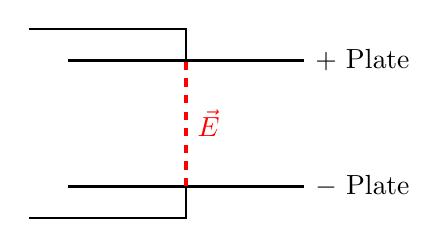
\begin{tikzpicture}[>=Stealth, thick]
        % Capacitor plates
        \draw [very thick] (-1.5,0.8) -- (1.5,0.8) node[right] {$+$ Plate};
        \draw [very thick] (-1.5,-0.8) -- (1.5,-0.8) node[right] {$-$ Plate};
        % Battery or lines
        \draw (0,0.8) -- (0,1.2) -- (-2,1.2);
        \draw (0,-0.8) -- (0,-1.2) -- (-2,-1.2);
        \draw [dashed, red, ultra thick] (0,-0.8) -- (0,0.8) node[midway, right] {$\vec{E}$};
    \end{tikzpicture}
\end{center}

Current exists in wires.
But between capacitor plates:
\[ I = 0 \]
(no conduction current).

Yet magnetic field still exists. This creates a contradiction.

\subsection*{Maxwell's Idea}
Maxwell proposed that a changing electric field behaves like a current.
This is called:
\begin{tcolorbox}[colback=RoyalBlue!5!white, colframe=RoyalBlue]
    \[ \text{Displacement Current} \]
\end{tcolorbox}

\subsection*{Electric Flux}
Electric flux:
\begin{tcolorbox}[colback=RoyalBlue!5!white, colframe=RoyalBlue]
    \[ \phi_E = \int \vec{E} \cdot d\vec{S} \]
\end{tcolorbox}

\subsection*{Displacement Current}
Maxwell defined
\begin{tcolorbox}[colback=RoyalBlue!5!white, colframe=RoyalBlue]
    \[ I_d = \epsilon_0 \frac{d\phi_E}{dt} \]
\end{tcolorbox}

\subsection*{Displacement Current Density}
\begin{tcolorbox}[colback=RoyalBlue!5!white, colframe=RoyalBlue]
    \[ J_d = \epsilon_0 \frac{\partial E}{\partial t} \]
\end{tcolorbox}

\subsection*{Modification of Ampere's Law}
Original Law:
\[ \oint \vec{B} \cdot d\vec{l} = \mu_0 I \]

Maxwell added displacement current term. Thus
\[ \oint \vec{B} \cdot d\vec{l} = \mu_0(I + I_d) \]
Substituting
\[ I_d = \epsilon_0 \frac{d\phi_E}{dt} \]
we get
\begin{tcolorbox}[colback=RoyalBlue!5!white, colframe=RoyalBlue]
    \[ \oint \vec{B} \cdot d\vec{l} = \mu_0 I + \mu_0\epsilon_0\frac{d\phi_E}{dt} \]
\end{tcolorbox}

\subsection*{Final Result}
\begin{tcolorbox}[colback=RoyalBlue!5!white, colframe=RoyalBlue]
    \[ \oint \vec{B} \cdot d\vec{l} = \mu_0 I + \mu_0\epsilon_0\frac{d\phi_E}{dt} \]
\end{tcolorbox}
This is called the Ampere-Maxwell Equation.

\subsection*{Differential Form}
Using Stokes' theorem,
\begin{tcolorbox}[colback=RoyalBlue!5!white, colframe=RoyalBlue]
    \[ \nabla \times \vec{B} = \mu_0\vec{J} + \mu_0\epsilon_0\frac{\partial\vec{E}}{\partial t} \]
\end{tcolorbox}

\subsection*{Physical Significance}
Magnetic field can be produced by:
Conduction Current \( I \) and Changing Electric Field \( \frac{\partial E}{\partial t} \).

\subsection*{Exam Ending Line}
Hence Maxwell removed the inconsistency in Ampere's law by introducing displacement current and obtained
\begin{tcolorbox}[colback=RoyalBlue!5!white, colframe=RoyalBlue]
    \[ \oint \vec{B} \cdot d\vec{l} = \mu_0 I + \mu_0\epsilon_0\frac{d\phi_E}{dt} \]
\end{tcolorbox}

\section*{Summary of Key Derivations}
\begin{tcolorbox}[colback=RoyalBlue!5!white, colframe=RoyalBlue, halign=center]
    \textbf{Register Complete \checkmark}
\end{tcolorbox}

This register contains the 18 high-yield derivations required for the E\&M curriculum:
\begin{enumerate}
    \item Gauss's Theorem
    \item Electric Field due to Infinite Line Charge
    \item Potential due to Dipole
    \item Electric Field due to Dipole
    \item Biot--Savart Law
    \item Magnetic Field due to Infinite Straight Wire
    \item Magnetic Field on Axis of Circular Coil
    \item Ampere's Circuital Law
    \item Magnetic Field Inside Solenoid
    \item Relation \( \mu = \mu_0(1+\chi) \)
    \item Faraday's Second Law
    \item Self-Inductance of Solenoid
    \item Continuity Equation
    \item Maxwell's Equations
    \item Thevenin's Theorem
    \item Maximum Power Transfer Theorem
    \item Mutual Inductance of Two Coaxial Solenoids
    \item Displacement Current \& Ampere-Maxwell Law
\end{enumerate}
All major analytical proofs across PYQ Sets 1, 2, and 3 are successfully detailed.

\end{document}
